\documentclass{standalone}
\usepackage{tikz}
\usetikzlibrary{patterns, positioning}

\begin{document}
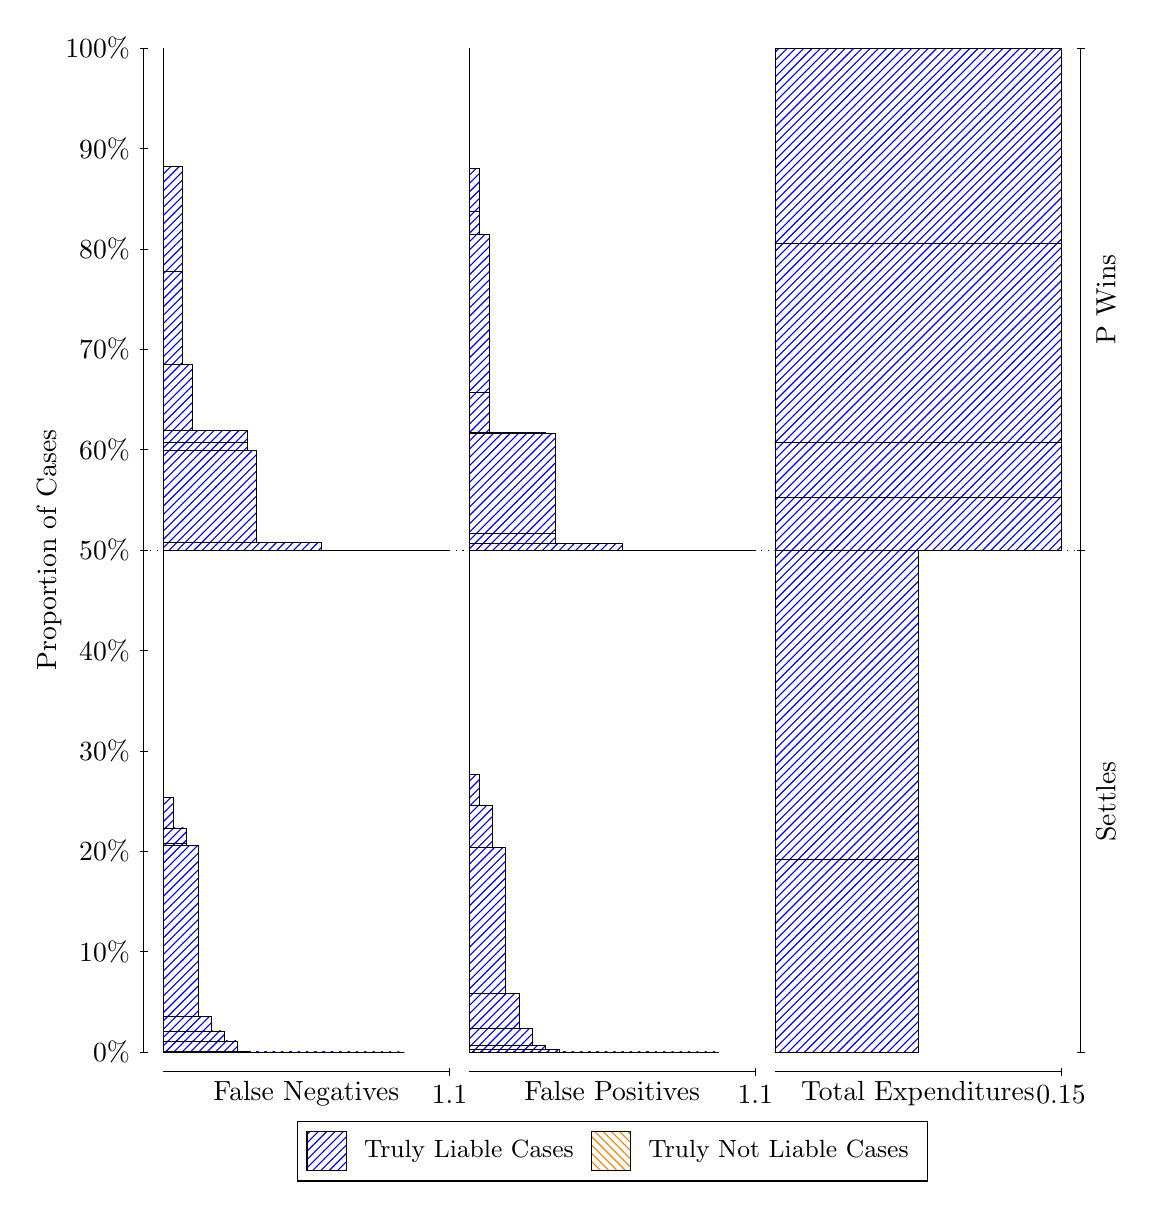
\begin{tikzpicture}
\draw[black, very thin] (1.5,1.75) -- (1.5,14.5);
\node[rotate=90, anchor=center] at (0.3, 8.125) {Proportion of Cases};
\draw[black, very thin] (1.45,1.75) -- (1.55,1.75);
\node[anchor=east] at (1.45, 1.75) {0\%};
\draw[black, very thin] (1.45,3.025) -- (1.55,3.025);
\node[anchor=east] at (1.45, 3.025) {10\%};
\draw[black, very thin] (1.45,4.3) -- (1.55,4.3);
\node[anchor=east] at (1.45, 4.3) {20\%};
\draw[black, very thin] (1.45,5.575) -- (1.55,5.575);
\node[anchor=east] at (1.45, 5.575) {30\%};
\draw[black, very thin] (1.45,6.85) -- (1.55,6.85);
\node[anchor=east] at (1.45, 6.85) {40\%};
\draw[black, very thin] (1.45,8.125) -- (1.55,8.125);
\node[anchor=east] at (1.45, 8.125) {50\%};
\draw[black, very thin] (1.45,9.4) -- (1.55,9.4);
\node[anchor=east] at (1.45, 9.4) {60\%};
\draw[black, very thin] (1.45,10.675) -- (1.55,10.675);
\node[anchor=east] at (1.45, 10.675) {70\%};
\draw[black, very thin] (1.45,11.95) -- (1.55,11.95);
\node[anchor=east] at (1.45, 11.95) {80\%};
\draw[black, very thin] (1.45,13.225) -- (1.55,13.225);
\node[anchor=east] at (1.45, 13.225) {90\%};
\draw[black, very thin] (1.45,14.5) -- (1.55,14.5);
\node[anchor=east] at (1.45, 14.5) {100\%};

\draw[black, very thin] (13.4,1.75) -- (13.4,14.5);
\draw[black, very thin] (13.35,1.75) -- (13.45,1.75);
\node[anchor=west] at (13.35, 1.75) {};
\draw[black, very thin] (13.35,8.1159) -- (13.45,8.1159);
\node[anchor=west] at (13.35, 8.1159) {};
\draw[black, very thin] (13.35,14.5) -- (13.45,14.5);
\node[anchor=west] at (13.35, 14.5) {};

\draw[black, very thin, pattern color=blue, pattern=north east lines] (1.75,1.75) rectangle (4.8118,1.75);
\draw[black, very thin, pattern color=blue, pattern=north east lines] (1.75,1.75) rectangle (4.4852,1.75);
\draw[black, very thin, pattern color=blue, pattern=north east lines] (1.75,1.75) rectangle (4.1586,1.75);
\draw[black, very thin, pattern color=blue, pattern=north east lines] (1.75,1.75) rectangle (3.9953,1.75);
\draw[black, very thin, pattern color=blue, pattern=north east lines] (1.75,1.75) rectangle (3.832,1.75);
\draw[black, very thin, pattern color=blue, pattern=north east lines] (1.75,1.75) rectangle (3.6687,1.75);
\draw[black, very thin, pattern color=blue, pattern=north east lines] (1.75,1.75) rectangle (3.5054,1.7503);
\draw[black, very thin, pattern color=blue, pattern=north east lines] (1.75,1.7503) rectangle (3.3421,1.7506);
\draw[black, very thin, pattern color=blue, pattern=north east lines] (1.75,1.7506) rectangle (3.1788,1.7508);
\draw[black, very thin, pattern color=blue, pattern=north east lines] (1.75,1.7508) rectangle (3.0155,1.7524);
\draw[black, very thin, pattern color=blue, pattern=north east lines] (1.75,1.7524) rectangle (2.8522,1.7556);
\draw[black, very thin, pattern color=blue, pattern=north east lines] (1.75,1.7556) rectangle (2.689,1.8905);
\draw[black, very thin, pattern color=blue, pattern=north east lines] (1.75,1.8905) rectangle (2.5257,2.0178);
\draw[black, very thin, pattern color=blue, pattern=north east lines] (1.75,2.0178) rectangle (2.3624,2.2045);
\draw[black, very thin, pattern color=blue, pattern=north east lines] (1.75,2.2045) rectangle (2.1991,4.3757);
\draw[black, very thin, pattern color=blue, pattern=north east lines] (1.75,4.3757) rectangle (2.0358,4.4043);
\draw[black, very thin, pattern color=blue, pattern=north east lines] (1.75,4.4043) rectangle (2.0358,4.5949);
\draw[black, very thin, pattern color=blue, pattern=north east lines] (1.75,4.5949) rectangle (1.8725,4.9855);
\draw[black, very thin, pattern color=orange, pattern=north west lines] (1.75,4.9855) rectangle (1.75,4.9855);
\draw[black, very thin, pattern color=blue, pattern=north east lines] (1.75,4.9855) rectangle (1.75,8.1159);
\draw[black, very thin, pattern color=blue, pattern=north east lines] (1.75,8.1159) rectangle (5.3833,8.1159);
\draw[black, very thin, pattern color=blue, pattern=north east lines] (1.75,8.1159) rectangle (4.5669,8.1171);
\draw[black, very thin, pattern color=blue, pattern=north east lines] (1.75,8.1171) rectangle (4.4444,8.1171);
\draw[black, very thin, pattern color=blue, pattern=north east lines] (1.75,8.1171) rectangle (3.7504,8.2202);
\draw[black, very thin, pattern color=blue, pattern=north east lines] (1.75,8.2202) rectangle (3.6279,8.2203);
\draw[black, very thin, pattern color=blue, pattern=north east lines] (1.75,8.2203) rectangle (2.9339,9.3914);
\draw[black, very thin, pattern color=blue, pattern=north east lines] (1.75,9.3914) rectangle (2.8114,9.4925);
\draw[black, very thin, pattern color=blue, pattern=north east lines] (1.75,9.4925) rectangle (2.8114,9.6402);
\draw[black, very thin, pattern color=blue, pattern=north east lines] (1.75,9.6402) rectangle (2.1174,10.486);
\draw[black, very thin, pattern color=blue, pattern=north east lines] (1.75,10.486) rectangle (1.9949,11.66);
\draw[black, very thin, pattern color=blue, pattern=north east lines] (1.75,11.66) rectangle (1.9949,12.998);
\draw[black, very thin, pattern color=orange, pattern=north west lines] (1.75,12.998) rectangle (1.75,12.998);
\draw[black, very thin, pattern color=blue, pattern=north east lines] (1.75,12.998) rectangle (1.75,14.5);
\draw[black, very thin, pattern color=orange, pattern=north west lines] (5.6333,1.75) rectangle (8.8019,1.75);
\draw[black, very thin, pattern color=blue, pattern=north east lines] (5.6333,1.75) rectangle (8.8019,1.75);
\draw[black, very thin, pattern color=orange, pattern=north west lines] (5.6333,1.75) rectangle (8.126,1.75);
\draw[black, very thin, pattern color=blue, pattern=north east lines] (5.6333,1.75) rectangle (8.126,1.75);
\draw[black, very thin, pattern color=blue, pattern=north east lines] (5.6333,1.75) rectangle (7.957,1.75);
\draw[black, very thin, pattern color=orange, pattern=north west lines] (5.6333,1.75) rectangle (7.788,1.75);
\draw[black, very thin, pattern color=blue, pattern=north east lines] (5.6333,1.75) rectangle (7.788,1.75);
\draw[black, very thin, pattern color=orange, pattern=north west lines] (5.6333,1.75) rectangle (7.45,1.75);
\draw[black, very thin, pattern color=blue, pattern=north east lines] (5.6333,1.75) rectangle (7.45,1.7501);
\draw[black, very thin, pattern color=blue, pattern=north east lines] (5.6333,1.7501) rectangle (7.281,1.7501);
\draw[black, very thin, pattern color=orange, pattern=north west lines] (5.6333,1.7501) rectangle (7.112,1.7501);
\draw[black, very thin, pattern color=blue, pattern=north east lines] (5.6333,1.7501) rectangle (7.112,1.7521);
\draw[black, very thin, pattern color=blue, pattern=north east lines] (5.6333,1.7521) rectangle (6.943,1.7521);
\draw[black, very thin, pattern color=orange, pattern=north west lines] (5.6333,1.7521) rectangle (6.774,1.7521);
\draw[black, very thin, pattern color=blue, pattern=north east lines] (5.6333,1.7521) rectangle (6.774,1.7841);
\draw[black, very thin, pattern color=blue, pattern=north east lines] (5.6333,1.7841) rectangle (6.605,1.8363);
\draw[black, very thin, pattern color=orange, pattern=north west lines] (5.6333,1.8363) rectangle (6.436,1.8363);
\draw[black, very thin, pattern color=blue, pattern=north east lines] (5.6333,1.8363) rectangle (6.436,2.0518);
\draw[black, very thin, pattern color=blue, pattern=north east lines] (5.6333,2.0518) rectangle (6.436,2.0531);
\draw[black, very thin, pattern color=blue, pattern=north east lines] (5.6333,2.0531) rectangle (6.2671,2.4922);
\draw[black, very thin, pattern color=orange, pattern=north west lines] (5.6333,2.4922) rectangle (6.0981,2.4922);
\draw[black, very thin, pattern color=blue, pattern=north east lines] (5.6333,2.4922) rectangle (6.0981,4.3445);
\draw[black, very thin, pattern color=blue, pattern=north east lines] (5.6333,4.3445) rectangle (6.0981,4.3448);
\draw[black, very thin, pattern color=blue, pattern=north east lines] (5.6333,4.3448) rectangle (5.9291,4.8804);
\draw[black, very thin, pattern color=blue, pattern=north east lines] (5.6333,4.8804) rectangle (5.7601,5.271);
\draw[black, very thin, pattern color=blue, pattern=north east lines] (5.6333,5.271) rectangle (5.6333,8.1159);
\draw[black, very thin, pattern color=orange, pattern=north west lines] (5.6333,8.1159) rectangle (9.2667,8.1159);
\draw[black, very thin, pattern color=blue, pattern=north east lines] (5.6333,8.1159) rectangle (9.2667,8.1159);
\draw[black, very thin, pattern color=orange, pattern=north west lines] (5.6333,8.1159) rectangle (8.4217,8.1159);
\draw[black, very thin, pattern color=blue, pattern=north east lines] (5.6333,8.1159) rectangle (8.4217,8.1168);
\draw[black, very thin, pattern color=orange, pattern=north west lines] (5.6333,8.1168) rectangle (7.5767,8.1168);
\draw[black, very thin, pattern color=blue, pattern=north east lines] (5.6333,8.1168) rectangle (7.5767,8.2079);
\draw[black, very thin, pattern color=orange, pattern=north west lines] (5.6333,8.2079) rectangle (7.45,8.2079);
\draw[black, very thin, pattern color=blue, pattern=north east lines] (5.6333,8.2079) rectangle (7.45,8.2079);
\draw[black, very thin, pattern color=orange, pattern=north west lines] (5.6333,8.2079) rectangle (6.7318,8.2079);
\draw[black, very thin, pattern color=blue, pattern=north east lines] (5.6333,8.2079) rectangle (6.7318,8.3402);
\draw[black, very thin, pattern color=blue, pattern=north east lines] (5.6333,8.3402) rectangle (6.7318,9.6092);
\draw[black, very thin, pattern color=orange, pattern=north west lines] (5.6333,9.6092) rectangle (6.605,9.6092);
\draw[black, very thin, pattern color=blue, pattern=north east lines] (5.6333,9.6092) rectangle (6.605,9.6184);
\draw[black, very thin, pattern color=blue, pattern=north east lines] (5.6333,9.6184) rectangle (5.8868,10.123);
\draw[black, very thin, pattern color=blue, pattern=north east lines] (5.6333,10.123) rectangle (5.8868,12.13);
\draw[black, very thin, pattern color=orange, pattern=north west lines] (5.6333,12.13) rectangle (5.7601,12.13);
\draw[black, very thin, pattern color=blue, pattern=north east lines] (5.6333,12.13) rectangle (5.7601,12.428);
\draw[black, very thin, pattern color=blue, pattern=north east lines] (5.6333,12.428) rectangle (5.7601,12.976);
\draw[black, very thin, pattern color=blue, pattern=north east lines] (5.6333,12.976) rectangle (5.6333,14.5);
\draw[black, very thin, pattern color=orange, pattern=north west lines] (9.5167,1.75) rectangle (11.333,1.75);
\draw[black, very thin, pattern color=blue, pattern=north east lines] (9.5167,1.75) rectangle (11.333,4.1968);
\draw[black, very thin, pattern color=orange, pattern=north west lines] (9.5167,4.1968) rectangle (11.333,4.1968);
\draw[black, very thin, pattern color=blue, pattern=north east lines] (9.5167,4.1968) rectangle (11.333,8.1159);
\draw[black, very thin, pattern color=orange, pattern=north west lines] (9.5167,8.1159) rectangle (13.15,8.1159);
\draw[black, very thin, pattern color=blue, pattern=north east lines] (9.5167,8.1159) rectangle (13.15,8.795);
\draw[black, very thin, pattern color=orange, pattern=north west lines] (9.5167,8.795) rectangle (13.15,8.795);
\draw[black, very thin, pattern color=blue, pattern=north east lines] (9.5167,8.795) rectangle (13.15,9.4939);
\draw[black, very thin, pattern color=orange, pattern=north west lines] (9.5167,9.4939) rectangle (13.15,9.4939);
\draw[black, very thin, pattern color=blue, pattern=north east lines] (9.5167,9.4939) rectangle (13.15,12.021);
\draw[black, very thin, pattern color=orange, pattern=north west lines] (9.5167,12.021) rectangle (13.15,12.021);
\draw[black, very thin, pattern color=blue, pattern=north east lines] (9.5167,12.021) rectangle (13.15,14.5);
\draw[black, dotted] (1.5,8.1159) -- (13.4,8.1159);
\draw[black, very thin] (1.75,1.5) -- (5.3833,1.5);
\node[anchor=north] at (3.5667, 1.5) {False Negatives};
\draw[black, very thin] (5.3833,1.45) -- (5.3833,1.55);
\node[anchor=north] at (5.3833, 1.45) {1.1};

\draw[black, very thin] (5.6333,1.5) -- (9.2667,1.5);
\node[anchor=north] at (7.45, 1.5) {False Positives};
\draw[black, very thin] (9.2667,1.45) -- (9.2667,1.55);
\node[anchor=north] at (9.2667, 1.45) {1.1};

\draw[black, very thin] (9.5167,1.5) -- (13.15,1.5);
\node[anchor=north] at (11.333, 1.5) {Total Expenditures};
\draw[black, very thin] (13.15,1.45) -- (13.15,1.55);
\node[anchor=north] at (13.15, 1.45) {0.15};

\node[black, centered, rotate=90] at (13.72, 4.933) {Settles};
\node[black, centered, rotate=90] at (13.72, 11.308) {P Wins};

\draw (7.449999999999999,1.5) node[draw=none] (baseCoordinate) {};
\begin{scope}[align=center]
        \matrix[scale=0.5, draw=black, below=0.5cm of baseCoordinate, nodes={draw}, column sep=0.1cm]{
            \node[rectangle, draw, minimum width=0.5cm, minimum height=0.5cm, pattern=north east lines, pattern color=blue] {}; &
            \node[draw=none, font=\small] (B) {Truly Liable Cases}; &
            \node[rectangle, draw, minimum width=0.5cm, minimum height=0.5cm, pattern=north west lines, pattern color=orange] {}; &
            \node[draw=none, font=\small] (B) {Truly Not Liable Cases}; \\
            };
\end{scope}

\end{tikzpicture}
\end{document}